\chap{复平面}
\section{介绍}
一些学科的历史往往是令人兴奋的读物,尤其是在对日期或先有技术存在争议的情况下。澄清谁在别人之前做了某事是历史学家的工作,他们可以帮助揭示谁应该为某一事件负责,谁应该居功至伟。要从日记、书籍和私人信件中理清事件的来龙去脉,并将它们按时间顺序排列在一起,需要具备学科知识、坚韧的毅力和客观的分析。

对于大多数研究学科来说,有两个日期对于确定优先权非常重要:论文提交发表的日期和被接受的论文发表的日期。这样的协议似乎是一个公平的方案,但前提是要有一个高效的邮政系统、一个公正的同行评审系统,以及其他许多条件。

在数学和科学领域,一些研究人员并不总是有信心将一个萌芽的想法发表出来,如果不发表,这个想法要么留在他们的脑海里,要么放在他们桌上的笔记本里,在研究人员死后可能被发现,也可能不被发现。对研究人员来说,不幸的是,人的脑袋并不是历史学家方便的信息存放处!

有时,数学论文会出现在与其他学科相关的期刊上,可以理解的是,这些期刊并不一定受到数学界的监督。同样,历史学家或好奇的学者通过巧妙的侦查工作,也会将复杂的优先权、归属问题浮出水面,在某些情况下,还会引起令人不快的剽窃嫌疑。

复数平面的发明是一个完美的例子,它说明了当数学思想的官方发布渠道被 "双关 "时,发明者会遇到怎样的严重问题。让我们看看发生了什么。

\section{一些历史}
一切始于 1813 年,瑞士业余数学家让-罗伯特-阿尔冈(Jean-Robert Argand,1768-1822 年)在他私人资助的一本 "小册子 "中发表了他关于复数几何解释的想法:关于几何构造中虚量表示方法的论文(Essai sur une manière de représenter les quantités imaginaires dans les constructions géométriques)\cite{bib4-1}。

这本小册子并没有广泛传播,更糟糕的是,它并没有 Argand 的名字!1813 年,Jacques Français 在一篇论文中重新发表了复平面的想法,并要求最初想法的匿名作者透露自己的身份。Argand 站了出来,他的发明得到了认可,如今复平面被称为 Argand 图。1874 年,Gauthier-Villars 出版社出版了 Argand 著作的第二版\cite{bib4-2}。

当时,挪威测量学家卡斯帕-韦塞尔(Caspar Wessel,1745-1818 年)一直在对丹麦进行三角测量,并开发数学技术来简化工作,但 Argand 和其他人都不知道。其中一个想法是添加矢量的原始想法,另一个是复数的几何解释。

1797 年, Wessel 在丹麦皇家学院的一次会议上提交了他的第一篇也是唯一一篇描述复平面的数学论文,并于 1799 年发表在学院的《备忘录》上。Wessel 的论文被数学界隐藏了近一个世纪,直到 1895 年才被丹麦数学家索福斯-克里斯蒂安-朱尔(Sophus Christian Juel,1855-1935 年)发现。尽管现在大家都认为 Wessel 是第一个发明复数平面的人,但复数平面仍以 Argand 的名字命名。

但这并没有结束!苏格兰数学家彼得-加斯里-泰特( Peter Guthrie Tait,1831-1901 年)在他的著作《四元数初论》中写道:"在十七世纪末,沃利斯提出用一条线来表示一元二次方程的不可能根:

\begin{CJK}{UTF8}{gkai}
    Wallis 在十七世纪末,提出了表示一元二次方程不可能的根的方法,即离开如果是真实的根就会在其上的直线。他的构造等同于把 $\sqrt{-1}$ 看作一条垂直于实数测量线的有向单位线。\cite{bib4-3}
\end{CJK}

约翰-沃利斯(John Wallis,1616-1703 年)是一位天才的英国数学家\cite{bib4-4},人们相信, Argand, Warren和其他人扩展了 Wallis 和 De Moivre 的成果,他们在复平面方面做了一些早期工作。

\section{复平面}
杰出的瑞士数学家莱昂哈德-欧拉(Leonhard Euler, 1707-1783 年)是与复数的发展有关的人物之一。欧拉证明了复数的特性:
$$
    e^{i \theta}=\cos \theta+i \sin \theta
$$
而当 $\theta=\pi$ 出现时,数学中最美丽的公式之一就出现了:
$$
    e^{i \pi}=-1
$$
或
$$
    e^{i \pi}+1=0
$$
这整合了五个重要常数:$0,1, e, \pi$ 和 $i$,以及基本算术运算:加法、乘法和指数运算。

当 $\theta=\pi / 2$ 时,这个公式的另一个结果就产生了:
$$
    e^{i \pi / 2}=\cos \left(\frac{\pi}{2}\right)+i \sin \left(\frac{\pi}{2}\right)=i
$$
因此\footnote{译者注,和网友讨论,并不止这一种结果,正确的结果应该如此:
    \begin{align*}
        \begin{aligned}
            i   & =  \cos (\frac{\pi}{2}+2k\pi)+i\sin(\frac{\pi}{2}+2k\pi) \\
                & =e^{i({\pi/2}+2k\pi)},\qquad k\in \mathbb{Z}             \\
            i^i & = e^{-(\pi/2+2k\pi)},\qquad k\in \mathbb{Z}              \\
        \end{aligned}
    \end{align*}

    是一个完全的实数的实数幂函数,对应多个值,感谢网友“天津-莲子粥(嵌入式)”。}
$$
    \begin{aligned}
        i^{i} & =\left(e^{i \pi / 2}\right)^{i} \\
              & =e^{i^{2} \pi / 2}              \\
              & =e^{-\pi / 2}                   \\
              & \approx 0.207879576 .
    \end{aligned}
$$
这表明虚数单位自身的幂等于一个实数!\footnote{译者注,参考上一条脚注,应该是一系列实数。}

\begin{figure}[htbp]
    \centering
    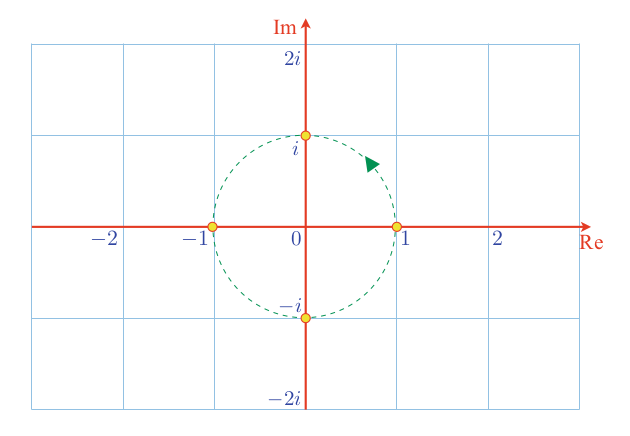
\includegraphics[max width=0.55\textwidth, center]{4.1}
    \caption[short]{带单位圆的复平面}
    \label{fig:4.1}
\end{figure}

在第三章中,我们看到虚$i$的幂产生了两个序列 $(1, i,-1,-i, 1, \ldots)$ 和 $(1,-i,-1, i, 1, \ldots)$ ,它们与分别沿逆时针和顺时针方向绕笛卡尔轴旋转时产生的模式$(x, y,-x,-y, x, \ldots)$ 和 $(x,-y,-x, y, x, \ldots)$ 惊人地相似。这种相似并非巧合,因为复数属于一个叫做复平面的二维平面,我们现在将描述它。

如图\ref{fig:4.1}所示,复数平面使我们能够用横轴记录实部、纵轴记录虚部来直观地表示复数。

该图还显示了一个单位半径的圆经过$1, i,-1,-i$,这是与$i$的幂次增加相关的序列。我们可以看到$i^{0}=1, i^{1}=i, i^{2}=-1, i^{3}=-i$和$i^{4}=1$的位置,这表明乘以$i$相当于旋转$90^{\circ}$。

为了演示这种旋转效应,图\ref{fig:4.2}给出了带四个复数的复平面:
$$
    p=2+i, \quad q=-1+2 i, \quad r=-2-i, \quad s=1-2 i
$$
它们之间的距离是$90^{\circ}$。
\begin{figure}[htbp]
    \centering
    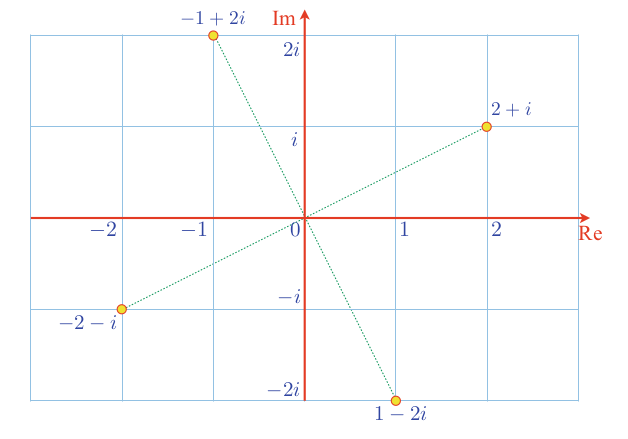
\includegraphics[max width=0.55\textwidth, center]{4.2}
    \caption[short]{标记4个复数的复平面}
    \label{fig:4.2}
\end{figure}

通过将点$p$乘以$i$,将点$p$旋转$90^{\circ}$到$q$:
$$
    \begin{aligned}
        i(2+i) & =2 i+i^{2} \\
               & =-1+2 i .
    \end{aligned}
$$
通过乘以$i$,将点$q$再旋转$90^{\circ}$到$r$:
$$
    \begin{aligned}
        i(-1+2 i) & =-i+2 i^{2} \\
                  & =-2-i
    \end{aligned}
$$
通过乘以$i$,将点$r$再旋转$90^{\circ}$到$s$:
$$
    \begin{aligned}
        i(-2-i) & =-2 i-i^{2} \\
                & =1-2 i
    \end{aligned}
$$
最后,通过乘以$i$,将$s$旋转$90^{\circ}$回到$p$:
$$
    \begin{aligned}
        i(1-2 i) & =i-2 i^{2} \\
                 & =2+i
    \end{aligned}
$$

在第三章中,我们还发现与增加负幂相关的序列:$(1,-i,-1, i, \ldots)$是顺时针方向的旋转,并且意味着将一个复数除以$i$使其顺时针旋转$90^{\circ}$。然而,我们证明了$i^{-1}=-i$,用$-i$乘以一个复数要比用$i$除以它容易得多。所以让我们重复上面的练习来证明这一点。

点$p$乘以$-i$被旋转$-90^{\circ}$到$s$:
$$
    \begin{aligned}
        -i(2+i) & =-2 i-i^{2} \\
                & =1-2 i .
    \end{aligned}
$$
点$s$再乘以$-i$旋转$-90^{\circ}$到$r$:
$$
    \begin{aligned}
        -i(1-2 i) & =-i+2 i^{2} \\
                  & =-2-i .
    \end{aligned}
$$
点$r$再乘以$-i$旋转$-90^{\circ}$到$q$,:
$$
    \begin{aligned}
        -i(-2-i) & =2 i+i^{2} \\
                 & =-1+2 i .
    \end{aligned}
$$
最后,点$q$乘以$-i$被旋转$-90^{\circ}$为$p$:
$$
    \begin{aligned}
        -i(-1+2 i) & =i-2 i^{2} \\
                   & =2+i .
    \end{aligned}
$$
因此,将一个复数旋转$\pm 90^{\circ}$,乘以$\pm i$。

在第3章中,我们看到$\sqrt{\pm i}$的根为
$$
    \begin{aligned}
         & \sqrt{+i}=\pm \frac{\sqrt{2}}{2}(1+i) \\
         & \sqrt{-i}=\pm \frac{\sqrt{2}}{2}(1-i)
    \end{aligned}
$$
\begin{figure}[htbp]
    \centering
    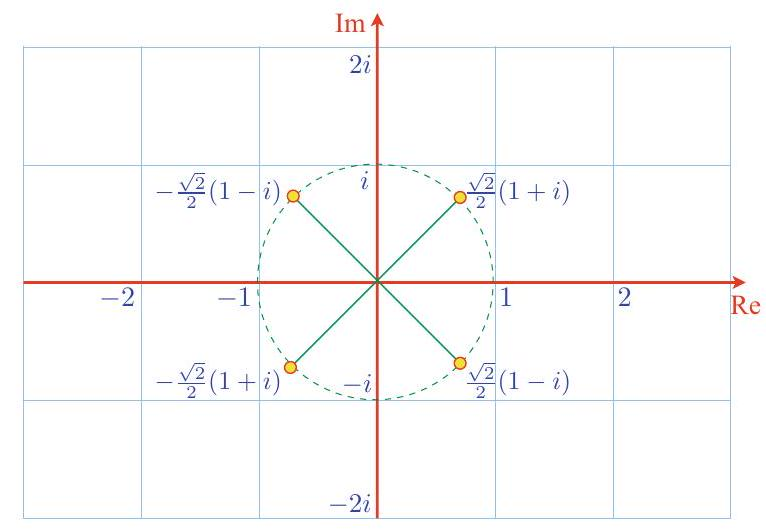
\includegraphics[max width=0.55\textwidth]{2023_04_20_41f1ceac5a31dc7d1b59g-071}
    \caption[short]{$\sqrt{ \pm i}$的复数根}
    \label{fig:4.3}
\end{figure}
如图\ref{fig:4.3}所示。请注意,每个根之间的距离为$180^{\circ}$,这表明角度与它们的作用有关。例如,$\sqrt{i}$的正根是$\sqrt{2} / 2(1+i)$,距离实轴为$45^{\circ}$。将这个根乘以它自己将它旋转到$i$轴上。同样,负根是$-\sqrt{2} / 2(1+i)$,与实轴的距离为$225^{\circ}$。将这个根乘以它自己将它$225^{\circ}$旋转到$i$轴。对于$\sqrt{-i}$的根也是如此。


这些观察似乎表明,我们可以构造一个能够将另一个复数旋转任何角度的复数。这是真的,我们接下来会讲到。

\section{极坐标表示法}
在复平面上放置一个复数,我们将得到极坐标表示法,在极坐标表示法中,从原点到复数形成一条直线,如图\ref{fig:4.4} 所示。这条线的长度是$r$,等于$\sqrt{a^{2}+b^{2}}$,这就是为什么复数的范数是用勾股定理定义的:
$$
    r=|z|=\sqrt{a^{2}+b^{2}}
$$
直线与实轴之间的角度$\theta$称为$z$的参数,表示为:
$$
    \arg (z)=\theta
$$
其中
$$
    \tan \theta=\frac{b}{a}
$$
\begin{align*}
    \text{第一象限:}        & a>0, b>0, & \theta=\arctan \left(\frac{b}{a}\right).       \\
    \text{第二第三象限:} & a<0,      &
    \theta=\arctan \left(\frac{b}{a}\right) +\pi.                                              \\
    \text{第四象限:}        & a>0, b<0, & \theta=\arctan \left(\frac{b}{a}\right)+2 \pi.
\end{align*}

\begin{figure}[htbp]
    \begin{center}
        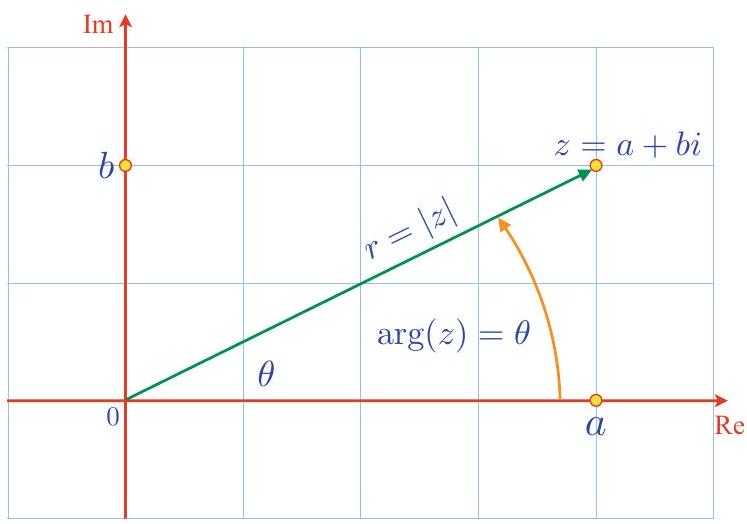
\includegraphics[max width=0.5\textwidth]{2023_04_20_41f1ceac5a31dc7d1b59g-072}
    \end{center}
    \caption[short]{复数的表示}
    \label{fig:4.4}
\end{figure}

由图\ref{fig:4.4}可知,$z$的水平分量为$r \cos \theta$,垂直分量为$r \sin \theta$,我们可以这样写
$$
    \begin{aligned}
        z & =a+b i                          \\
          & =r \cos \theta+r i \sin \theta  \\
          & =r(\cos \theta+i \sin \theta) .
    \end{aligned}
$$
如之前所述,欧拉的发现之一是$e^{\theta}, \sin \theta$和$\cos \theta$的幂级数的同一性:
$$
    e^{i \theta}=\cos \theta+i \sin \theta
$$
这样我们就可以写出
$$
    z=r e^{i \theta}
$$
有了这一发现,我们现在就可以用极坐标形式重新研究两个复数的积和商了。例如,给出以下复数:
$$
    \begin{aligned}
        z & =r e^{i \theta} \\
        w & =s e^{i \phi}
    \end{aligned}
$$
它们的乘积是
$$
    \begin{aligned}
        z w & =r s e^{i \theta} e^{i \phi}                  \\
            & =r s e^{i(\theta+\phi)}                       \\
            & =r s[\cos (\theta+\phi)+i \sin (\theta+\phi)]
    \end{aligned}
$$
因此,两个复数的乘积会产生第三个复数,其范数为
$$
    |z w|=r s
$$
且参数
$$
    \arg (z w)=\theta+\phi
$$
这里两个角度相加了。

接下来是商:
$$
    \begin{aligned}
        \frac{z}{w} & =\frac{r e^{i \theta}}{s e^{i \phi}}                  \\
                    & =\frac{r}{s} e^{i(\theta-\phi)}                       \\
                    & =\frac{r}{s}[\cos (\theta-\phi)+i \sin (\theta-\phi)]
    \end{aligned}
$$
它的范数是
$$
    \left|\frac{z}{w}\right|=\frac{r}{s}
$$
参数是
$$
    \arg \left(\frac{z}{w}\right)=\theta-\phi
$$
这里是两个角度相减了。

让我们举例说明这些公式。图\ref{fig:4.5}显示了两个复数:
$$
    \begin{gathered}
        z=2+2 i \\
        w=-1+i
    \end{gathered}
$$
其极坐标形式为
$$
    \begin{aligned}
        z & =2 \sqrt{2}\left(\cos 45^{\circ}+i \sin 45^{\circ}\right)=2 \sqrt{2} e^{i \pi / 4}   \\
        w & =\sqrt{2}\left(\cos 135^{\circ}+i \sin 135^{\circ}\right)=\sqrt{2} e^{i 3 \pi / 4} .
    \end{aligned}
$$
用普通的复代数,积zw是
$$
    z w=(2+2 i)(-1+i)=-4
$$


\begin{figure}[htbp]
    \begin{center}
        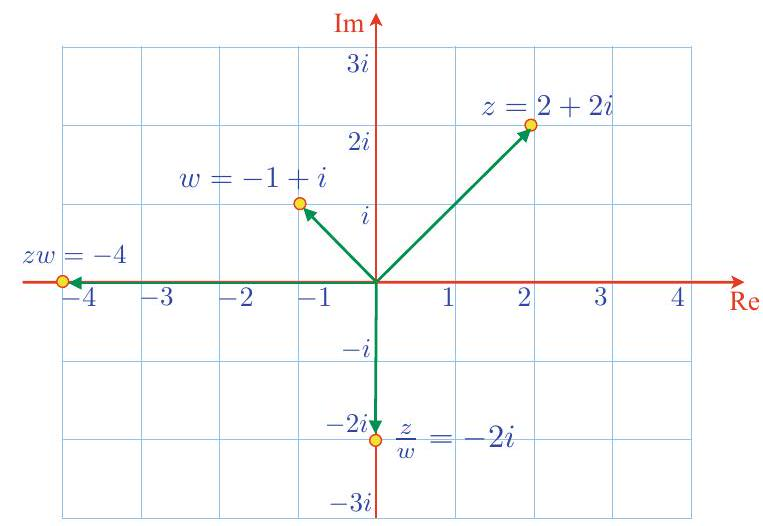
\includegraphics[max width=0.5\textwidth]{2023_04_20_41f1ceac5a31dc7d1b59g-074}
    \end{center}
    \caption[short]{两个复数的乘积和商}
    \label{fig:4.5}
\end{figure}

用极坐标形式:
$$
    \begin{aligned}
        |z w|      & =2 \sqrt{2} \sqrt{2}=4              \\
        \arg (z w) & =45^{\circ}+135^{\circ}=180^{\circ}
    \end{aligned}
$$
这编码了 -4 。
现在我们用普通复数代数计算商$z / w$,然后求极坐标形式。
$$
    \begin{aligned}
        \frac{z}{w} & =\frac{(2+2 i)}{(-1+i)} \frac{(-1-i)}{(-1-i)} \\
                    & =\frac{-2-2 i-2 i-2 i^{2}}{1+1}               \\
                    & =-2 i .
    \end{aligned}
$$
接下来,用极坐标形式
$$
    \begin{aligned}
        \left|\frac{z}{w}\right|      & =\frac{2 \sqrt{2}}{\sqrt{2}}=2      \\
        \arg \left(\frac{z}{w}\right) & =45^{\circ}-135^{\circ}=-90^{\circ}
    \end{aligned}
$$
这编码了复数$-2 i$。结果如图\ref{fig:4.5}所示。

我们也可以用欧拉公式计算$\sqrt{i}$如下:
$$
    e^{i \theta}=\cos \theta+i \sin \theta
$$
代入$\theta=\pi / 2$
$$
    e^{i \pi / 2}=\cos \left(\frac{\pi}{2}\right)+i \sin \left(\frac{\pi}{2}\right)=i
$$
两边开平方根,得到
$$
    \begin{aligned}
        \pm e^{i \pi / 4}                                                                 & =\sqrt{i} \\
        \pm\left[\cos \left(\frac{\pi}{4}\right)+i \sin \left(\frac{\pi}{4}\right)\right] & =\sqrt{i} \\
        \pm \frac{\sqrt{2}}{2}(1+i)                                                       & =\sqrt{i}
    \end{aligned}
$$
为求$\sqrt{-i}$,我们代入$\theta=-\pi / 2$:
$$
    \begin{aligned}
        e^{-i \pi / 2} & =\cos \left(-\frac{\pi}{2}\right)+i \sin \left(-\frac{\pi}{2}\right)=-i \\
                       & =\cos \left(\frac{\pi}{2}\right)-i \sin \left(\frac{\pi}{2}\right)=-i
    \end{aligned}
$$
两边开平方根,得到
$$
    \begin{aligned}
        \pm e^{-i \pi / 4}                                                                & =\sqrt{-i} \\
        \pm\left[\cos \left(\frac{\pi}{4}\right)-i \sin \left(\frac{\pi}{4}\right)\right] & =\sqrt{-i} \\
        \pm \frac{\sqrt{2}}{2}(1-i)                                                       & =\sqrt{-i}
    \end{aligned}
$$

使用类似的技术可以找到更高的根。

\section{转子}
极坐标形式表明了这样一个事实:将$z=r e^{i \theta}$与范数$r$相乘,再乘以$w=s e^{i \phi}$与范数$s$相乘,就产生了第三个复数,范数为$r s$。因此,为了避免缩放$z, w$必须有一个单位范数。在这种情况下,$w$充当转子。例如,将$4+5 i$乘以$1+0 i$使其保持未缩放和未旋转状态。但是,将$4+5 i$乘以$0+i$将其旋转为$90^{\circ}$而不进行任何缩放。

因此,要将 $2+2 i$ 旋转 $45^{\circ}$ ,必须乘以 $e^{i \pi / 4}$ :
$$
    \begin{aligned}
        e^{i \pi / 4}                  & =\cos 45^{\circ}+i \sin 45^{\circ}=\frac{\sqrt{2}}{2}(1+i) \\
        \frac{\sqrt{2}}{2}(1+i)(2+2 i) & =\frac{\sqrt{2}}{2} 4 i                                    \\
                                       & =2 \sqrt{2} i
    \end{aligned}
$$
因此,$e^{i \theta}$可以将任何复数旋转一个角度$\theta$。

要将复数 $x+y i$ 旋转一个角度 $\theta$,我们可以将其乘以转子 $cos \theta+i \sin \theta$
$$
    \begin{aligned}
        x^{\prime}+y^{\prime} i & =(\cos \theta+i \sin \theta)(x+y i)                         \\
                                & =x \cos \theta-y \sin \theta+i(x \sin \theta+y \cos \theta)
    \end{aligned}
$$
其矩阵形式为:
$$
    \left[\begin{array}{r}
            x^{\prime} \\
            i y^{\prime}
        \end{array}\right]=\left[\begin{array}{rr}
            \cos \theta & -\sin \theta \\
            \sin \theta & \cos \theta
        \end{array}\right]\left[\begin{array}{c}
            x \\
            i y
        \end{array}\right]
$$
在继续讨论之前,让我们先考虑一下转子的复共轭对旋转方向的影响,我们可以通过将 $x+y i$ 乘以转子 $cos \theta-$ $i \sin \theta$ 来做到这一点:
$$
    \begin{aligned}
        x^{\prime}+y^{\prime} i & =(\cos \theta-i \sin \theta)(x+y i)                          \\
                                & =x \cos \theta+y \sin \theta+i(-x \sin \theta+y \cos \theta)
    \end{aligned}
$$
其在矩阵形式中为
$$
    \left[\begin{array}{r}
            x^{\prime} \\
            i y^{\prime}
        \end{array}\right]=\left[\begin{array}{rr}
            \cos \theta  & \sin \theta \\
            -\sin \theta & \cos \theta
        \end{array}\right]\left[\begin{array}{c}
            x \\
            i y
        \end{array}\right]
$$
是围绕原点旋转 $-\theta$。

因此,我们将转子 $\mathbf{R}_{\theta}$ 及其共轭 $\mathbf{R}_{\theta}^{\dagger}$ 定义为

$$
    \begin{aligned}
         & \mathbf{R}_{\theta}=\cos \theta+i \sin \theta           \\
         & \mathbf{R}_{\theta}^{\dagger}=\cos \theta-i \sin \theta
    \end{aligned}
$$

其中 $\mathbf{R}_{\theta}$ 旋转 $+\theta$,而 $\mathbf{R}_{\theta}^{\dagger}$ 旋转 $-\theta$。注意匕首 $\dagger$ 符号的使用。

\section{总结}
在这一章中,我们发现了利用复平面对复数的图形化解释。欧拉公式 $e^{i \theta}=\cos \theta+i \sin \theta$ 允许我们将复数表示为$e$的虚次幂,从而使我们可以轻松地计算乘积和商。总之,这些想法让我们产生了转子的想法,而转子将使用四元数来开发。

\subsection{定义总结}
\begin{tcolorbox}[breakable, enhanced,title = {复数}]
    $$
        \begin{aligned}
            z   & =a+b i              \\
            |z| & =\sqrt{a^{2}+b^{2}}
        \end{aligned}
    $$
\end{tcolorbox}

\begin{tcolorbox}[breakable, enhanced,title = {极坐标形式}]
    $$
        \begin{aligned}
            z           & =r e^{i \theta}               \\
            z           & =r(\cos \theta+i \sin \theta) \\
            r           & =|z|                          \\
            \tan \theta & =b / a                        \\
            \theta      & =\arg (z) .
        \end{aligned}
    $$

    $$
        \begin{aligned}
            \text{第一象限:   }     & a>0, b>0  &  & \theta=\arctan \left(\frac{b}{a}\right).       \\
            \text{第二、第三象限: } & a<0,      &  & \theta=\arctan \left(\frac{b}{a}\right)+\pi.   \\
            \text{第四象限:  }      & a>0, b<0, &  & \theta=\arctan \left(\frac{b}{a}\right)+2 \pi.
        \end{aligned}
    $$
\end{tcolorbox}

\begin{tcolorbox}[breakable, enhanced,title = {乘积}]
    $$
        \begin{aligned}
            z   & =r e^{i \theta}                                 \\
            w   & =s e^{i \phi}                                   \\
            z w & =r s e^{i(\theta+\phi)}                         \\
                & =r s[\cos (\theta+\phi)+i \sin (\theta+\phi)] .
        \end{aligned}
    $$
\end{tcolorbox}
\begin{tcolorbox}[breakable, enhanced,title = {商}]
    $$
        \begin{aligned}
            \frac{z}{w} & =\frac{r}{s} e^{i(\theta-\phi)}                         \\
                        & =\frac{r}{s}[\cos (\theta-\phi)+i \sin (\theta-\phi)] .
        \end{aligned}
    $$
\end{tcolorbox}

\begin{tcolorbox}[breakable, enhanced,title = {转子}]
    $$
        \begin{aligned}
             & \mathbf{R}_{\theta}=\cos \theta+i \sin \theta             \\
             & \mathbf{R}_{\theta}^{\dagger}=\cos \theta-i \sin \theta .
        \end{aligned}
    $$
\end{tcolorbox}



\section{样例}
下面是一些进一步运用上述思想的例子。在某些情况下,需要进行测试以确认结果。

\begin{myexample}{用 \boldmath $i$ 旋转复数}{theoexample}
从 $1+2 i$ 开始,将得到的复数乘以 $i$四次,并在复数平面上绘出结果。

将点 $p$ 旋转 $90^{\circ}$ 至 $q$ 是通过乘以 $i$,:
$$
    \begin{aligned}
        i(1+2 i) & =i+2 i^{2} \\
                 & =-2+i .
    \end{aligned}
$$
通过乘以 $i$,点 $q$ 又旋转了 $90^{\circ}$ 至 $r$ :
$$
    \begin{aligned}
        i(-2+i) & =-2 i+i^{2} \\
                & =-1-2 i .
    \end{aligned}
$$

通过乘以 $i$,点 $r$ 又旋转了 $90^{\circ}$ 至 $s$:
$$
    \begin{aligned}
        i(-1-2 i) & =-i-2 i^{2} \\
                  & =2-i .
    \end{aligned}
$$

最后,通过乘以 $i$,将点 $s$ 旋转 $90^{\circ}$ 回到 $p$:
$$
    \begin{aligned}
        i(2-i) & =2 i-i^{2} \\
               & =2+i .
    \end{aligned}
$$

图\ref{fig:4.6} 显示了由 $90^{\circ}$ 分隔的四个复数。
\end{myexample}

\begin{figure}[htbp]
    \centering
    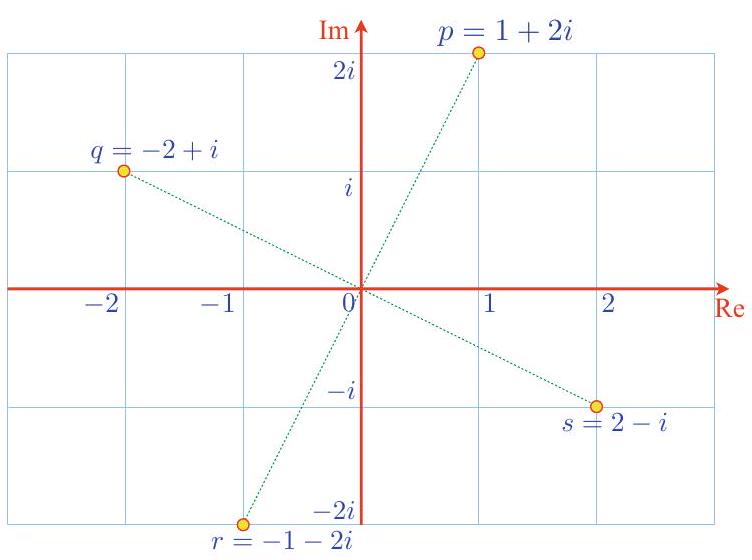
\includegraphics[max width=0.8\textwidth]{2023_04_20_41f1ceac5a31dc7d1b59g-078}
    \caption{有四个复数的复平面}
    \label{fig:4.6}
\end{figure}

\begin{myexample}{使用极坐标形式计算积和商}{theoexample}
用极坐标形式计算积 $z w$ 和商 $z / w$。
$$
    \begin{gathered}
        z=3+3 i \\
        w=-1-i .
    \end{gathered}
$$
乘积:
$$
    \begin{aligned}
        z          & =3 \sqrt{2}\left(\cos 45^{\circ}+i \sin 45^{\circ}\right)=3 \sqrt{2} e^{i \pi / 4} \\
        w          & =\sqrt{2}\left(\cos 225^{\circ}+i \sin 225^{\circ}\right)=\sqrt{2} e^{i 5 \pi / 4} \\
        |z w|      & =3 \sqrt{2} \sqrt{2}=6                                                             \\
        \arg (z w) & =45^{\circ}+225^{\circ}=270^{\circ}
    \end{aligned}
$$

编码复数 $-6 i$。

测试: 使用普通复数代数,乘积 $z w$ 是
$$
    z w=(3+3 i)(-1-i)=-6 i
$$

商:
$$
    \begin{aligned}
        |z|                           & =3 \sqrt{2}                         \\
        |w|                           & =\sqrt{2}                           \\
        \left|\frac{z}{w}\right|      & =3 \sqrt{2} / \sqrt{2}=3            \\
        \arg \left(\frac{z}{w}\right) & =45^{\circ}-225^{\circ}=180^{\circ}
    \end{aligned}
$$

编码复数 -3 。

测试: 使用普通复代数,商 $z / w$ 是
$$
    \begin{aligned}
        \frac{z}{w} & =\frac{(3+3 i)}{(-1-i)} \frac{(-1+i)}{(-1+i)} \\
                    & =\frac{-6}{2}                                 \\
                    & =-3
    \end{aligned}
$$
并与极坐标形式一致。
\end{myexample}


\begin{myexample}{设计一个旋转复数$30^{\circ}$的转子 }{theoexample}
设计一个转子,使复数在不缩放的情况下旋转 $30^{\circ}$ 。首先
$$
    e^{i \theta}=\cos \theta+i \sin \theta
$$

令 $\theta=30^{\circ}=\pi / 6$

$$
    \begin{aligned}
        e^{i \pi / 6} & =\cos 30^{\circ}+i \sin 30^{\circ} \\
                      & =\frac{\sqrt{3}}{2}+\frac{1}{2} i  \\
                      & =\frac{1}{2}(\sqrt{3}+i) .
    \end{aligned}
$$

测试: 让我们用这个转子将 $1+0 i$ 旋转三次,直到 $i$。
$$
    \begin{aligned}
        \frac{1}{2}(\sqrt{3}+i) \frac{1}{2}(\sqrt{3}+i) \frac{1}{2}(\sqrt{3}+i) 1 & =\frac{1}{8}(\sqrt{3}+i)(\sqrt{3}+i)(\sqrt{3}+i) \\
                                                                                  & =\frac{1}{8}(2+2 \sqrt{3} i)(\sqrt{3}+i)         \\
                                                                                  & =\frac{1}{8}(2 \sqrt{3}-2 \sqrt{3}+2 i+6 i)      \\
                                                                                  & =i
    \end{aligned}
$$
\end{myexample}

\begin{myexample}{设计一个将复数旋转 $-60^{\circ}$ 的转子}{theoexample}
设计一个转子,使复数在不缩放的情况下旋转$-60^{\circ}$。首先
$$
    e^{i \theta}=\cos \theta+i \sin \theta
$$

令 $\theta=-60^{\circ}=-\pi / 3$
$$
    \begin{aligned}
        e^{-i \pi / 3} & =\cos \left(-60^{\circ}\right)+i \sin \left(-60^{\circ}\right) \\
                       & =\frac{1}{2}-\frac{\sqrt{3}}{2} i                              \\
                       & =\frac{1}{2}(1-\sqrt{3} i)
    \end{aligned}
$$
\end{myexample}









\begin{thebibliography}{99}
    \bibitem{bib4-1} Argand, J.R.: \href{http://www-history.mcs.st-andrews.ac.uk/Mathematicians/Argand.html}{http://www-history.mcs.st-andrews.ac.uk/Mathematicians/Argand.html}
    \bibitem{bib4-2} Argand, J.R.: Essai sur une manière de représenter les quantités imaginaires dans les constructions géométriques, 2nd edn. Gauthier-Villars, Paris (1874)
    \bibitem{bib4-3} Tait, P.G.: Elementary Treatise on Quaternions. Cambridge University Press, Cambridge (1867)
    \bibitem{bib4-4} Wallis, J.: \href{http://www-history.mcs.st-andrews.ac.uk/Mathematicians/Wallis.html}{http://www-history.mcs.st-andrews.ac.uk/Mathematicians/Wallis.html}
\end{thebibliography}
